\documentclass[11pt,a4paper]{article}
\usepackage[T1]{fontenc}
\usepackage{graphicx}
\usepackage{amsmath,amssymb}
\usepackage{hyperref} % links, use \url{} or \href{url}{description}
% sett margin
\usepackage[left=3cm,right=3cm,top=3cm,bottom=3cm]{geometry}
\begin{document}
\title{Semester assignment TFY4240 - Aurora borealis}
\author{Arve Seljebu}
\thispagestyle{empty}
\begin{center}
\vspace{5mm}
\LARGE
\textbf{Semester assignment TFY4240 - Aurora borealis} \\
\Large
\vspace{5mm}
\textbf{by} \\
\vspace{5mm}
\large
\textbf{Arve Seljebu} \\
\vspace{5mm}
\textbf{7. november 2013} \\
\vspace{20mm}
\end{center}
\newpage
\tableofcontents
\thispagestyle{empty}
\setcounter{tocdepth}{2}
\newpage

%==================================================================
% Summary
%==================================================================
\section{Summary}
In this report you will read how charged particle trajectories travelling through a magnetic field from a dipole was calculated. This is similar to the solar wind hitting the earth. Since the magnetic field is not homogeneous, the paths of the particles form intresting patterns depending on the particle speed, weight, direction and charge.

%==============================================
% Theory
%==============================================
\section{Theory}
The earth's magnetic field is made by the current in the core. This models almost like a magnetic dipole, given by
% B-field
\begin{equation}
\label{equation.Bdip}
B_{dip}(r) = \frac{\mu_0}{4\pi} \frac{1}{r^3}[3(\textbf{m} \cdot \hat{\textbf{r} } ) \hat{\textbf{r}} -\textbf{m}].
\end{equation}
Where \textbf{m} is the magnetic dipole and \textbf{r} is the point where the magnetic field is measured. The origin is at the center of the dipole, here it's at earth center.

A charged particle moving in a magnetic field \textbf{B} will be subject to the magnetic force
\begin{equation}
\label{equation.forceMag}
F_{mag} = q(\textbf{v} \times \textbf{B}).
\end{equation}
Here \textbf{v} is the velocity of the particle, \textbf{B} is the B-field its travelling trough and $q$ is the charge of the particle.

The force on an object can also be described by Netown's second law
\begin{equation}
\label{equation.force}
F = m\textbf{a}.
\end{equation}

Here acceleration \textbf{a} describes how the velocity changes, giving the simple estimates
\begin{equation}
\label{equation.velocity}
\textbf{v}(t+\Delta t) = \textbf{v}(t) + \textbf{a}\Delta t \text
\end{equation}
\begin{equation}
\label{equation.position}
\textbf{r}(t+\Delta t) = \textbf{r}(t) + \textbf{v}\Delta t
\end{equation}
by Euler method.



%=============================================================
% Method
%=============================================================
\section{Method}
A reference system with x-axis towards the sun, z-axis perpendicular to earth orbit and origin at earth center was choosen. Python was used to do the calculations, mostly the library numpy. Mayavi was choosen for creating visualization.
\subsection{Calculating and representing the B-field}
A mesh grid containing all points in a cube was created. Then length and direction was calculated to each point in the grid, and then the B-field was calculated from equation \ref{equation.Bdip} numerically, without $\frac{\mu_0}{4\pi}$, earth radius set to 10 and the magnetic dipole $|\textbf{m}|$=2 tilted 13 degrees from z-axis.
To represent the B-field, both quiver and flow plots was tried. Quiver with scaled vectors and masked points gave the best representation. A video was made to represent the field by rotation around the axis and exporting pictures for each camera position.
\subsection{Particle trajectory}
Because of the nature of the problem, a numerical value representing weight, charge, velocity, strength of B-field, was choosen to make the trajectories easier to calculate.  The numerical value $k$ was put before $\textbf{v}\times\textbf{B}$, giving the numerical acceleration
\begin{equation}
\label{equation.numericalAcceleration}
\textbf{a} = k(\textbf{v}\times\textbf{B}).
\end{equation}
The time step was chosen by assuming the trajectory would behave correct when steps equals resolution of output. This was calculated by setting maximum distance to 50(5 times earth radius) and resolution to 720 pixels/points. This gives
\begin{equation}
\label{equation.dt}
\Delta t = \frac{50}{720|v|}.
\end{equation}
A loop through different $k$ values was done, and then evaluating the trajectories in 3D to pick a reasonable $k$ value. With reasonable meaning $k$ values that did give other trajectories then all through earth(force strength too low), or all particles bend off(force too high). Also, starting points $r_0$ from grid was evaluated, along with initial direction of the velocity parallel to x or z axis, or directly to the earth.
%==================================================================
% Discussion
%==================================================================
\section{Discussion}
The loop through different $k$ values with $v_0=\frac{400km/s}{6371km}10$ revealed that $k=200$ gave several entry points with roughly the same trajectory. The evaluation of starting points and velocity direction showed that particles coming directly towards the poles gave more particles with roughly the same trajectory. Therefore, these values was choosen as basis for the graphs discussed here.
\subsection{B-field}
A video of the B-field can be viewed at \href{http://youtube.com/watch?q=adsf}{youtube}. Under are B-field in 3D viewed from y or z axis.
\begin{center}
\begin{figure}[htbp] %[h]=here [t]=top [b]=bottom [p]=own page
\label{figure.B-field}
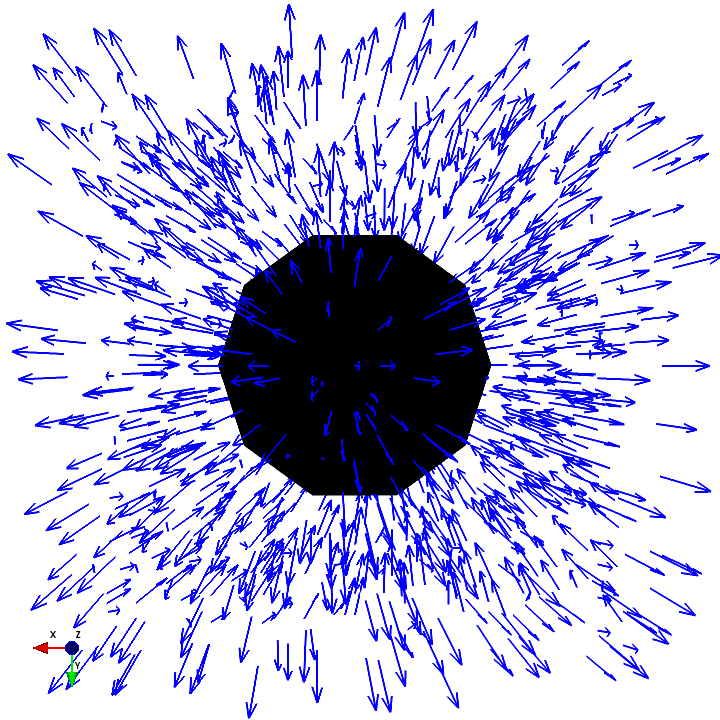
\includegraphics[width=0.5\textwidth]{xy-z_plus.png}
\caption{Magnetic field viewed with projection to the xy-plane. The complete direction is not easily read from this visualization, but it's easy to see that almost all points have a component of $\phi$ direction. As we will see in the next figure, it's the points that is directly above, below or beside the dipole that does not have any $\phi$ component. We can also read that the field is stronger closer to earth, and gets weaker when $r$ increases.}
\end{figure}
\end{center}

\begin{center}
\begin{figure}[htbp] %[h]=here [t]=top [b]=bottom [p]=own page
\label{figure.B-field}
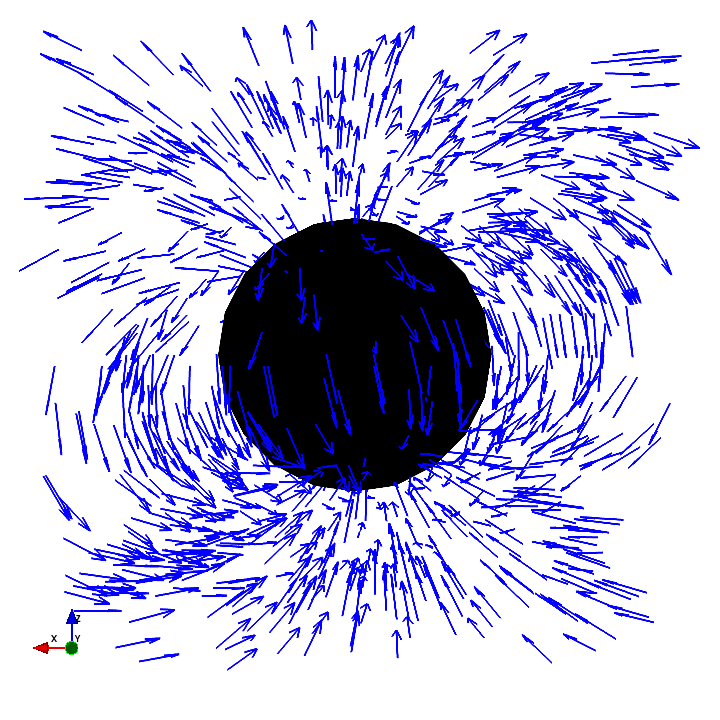
\includegraphics[width=0.5\textwidth]{xz-y_plus.png}
\caption{Here it's easier to see the z-component of the B-field. The field is tilted away from z-axis, as given by the magnetic dipole moment $\textbf{m}$.}
\end{figure}
\end{center}

\subsection{Proton trajectory}
An animation of some selected trajectories can be watched \href{here}{http://www.youtube.com/watch?v=Z0PT-oyBoS0}. Below are the visualizations that was picked as interesting.
\begin{center}
\begin{figure}[htbp] %[h]=here [t]=top [b]=bottom [p]=own page
\label{figure.B-field}
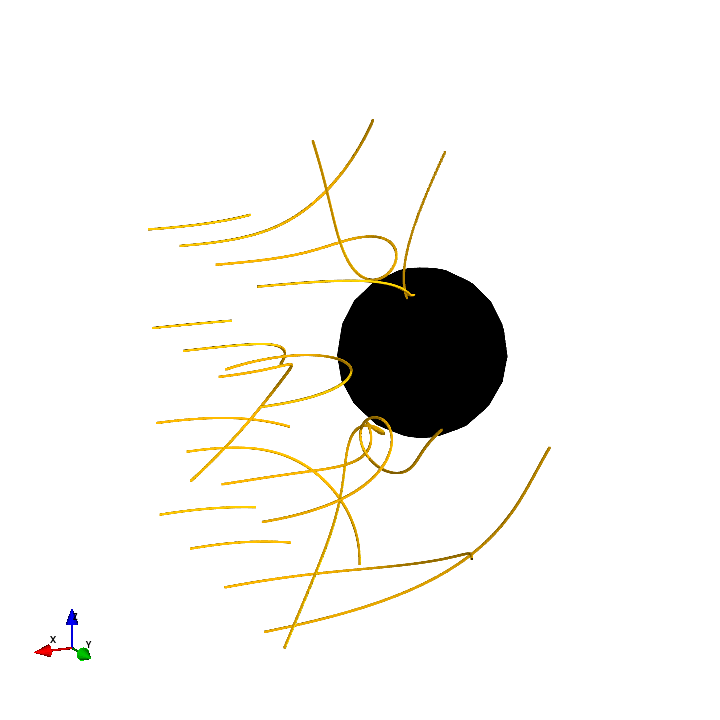
\includegraphics[width=0.5\textwidth]{x-straight.png}
\caption{}
\end{figure}
\end{center}
\begin{center}
\begin{figure}[htbp] %[h]=here [t]=top [b]=bottom [p]=own page
\label{figure.B-field}
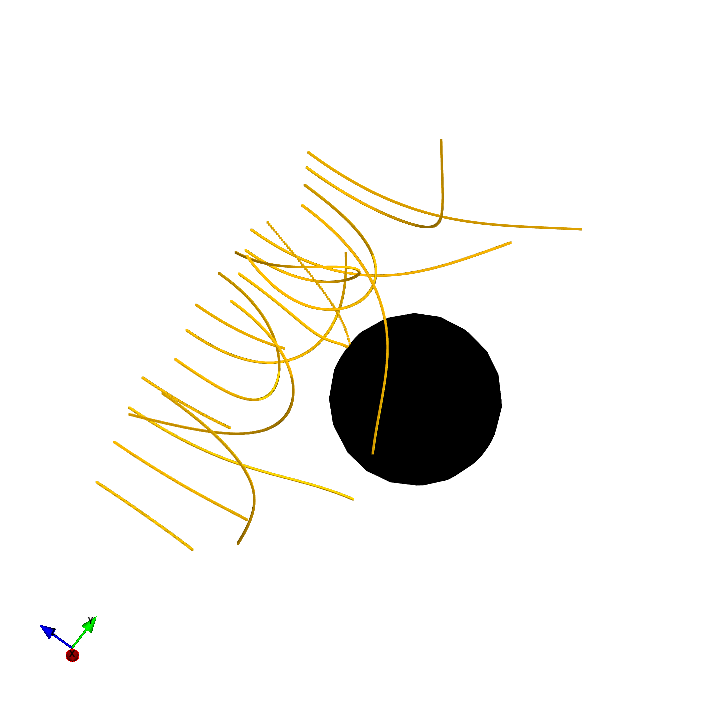
\includegraphics[width=0.5\textwidth]{z-straight.png}
\caption{}
\end{figure}
\end{center}
\begin{center}
\begin{figure}[htbp] %[h]=here [t]=top [b]=bottom [p]=own page
\label{figure.B-field}
\includegraphics[width=0.5\textwidth]{x-towards.png}
\caption{}
\end{figure}
\end{center}
\begin{center}
\begin{figure}[htbp] %[h]=here [t]=top [b]=bottom [p]=own page
\label{figure.B-field}
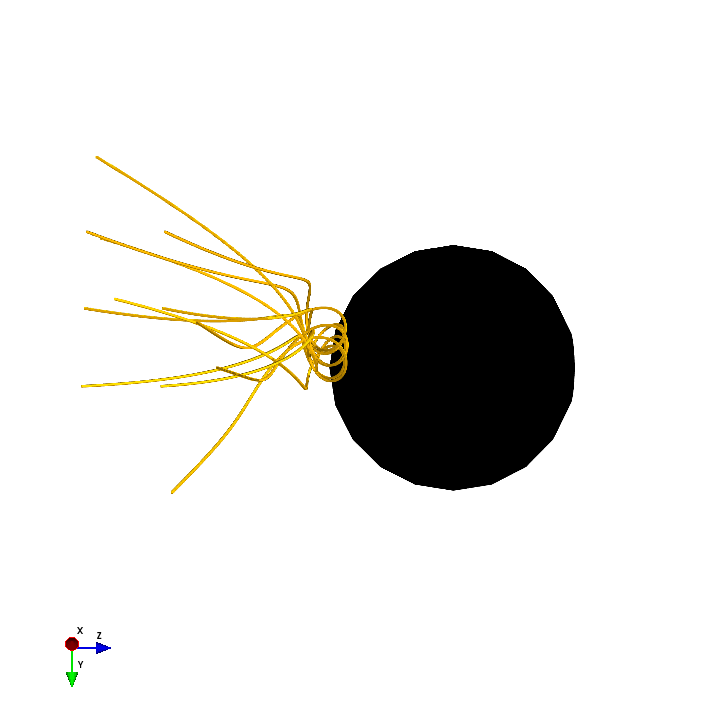
\includegraphics[width=0.5\textwidth]{toward-pole.png}
\caption{}
\end{figure}
\end{center}
%==================================================================
% Conclusion
%==================================================================

\section{Conclusion}

\end{document}
